\section{{\color{red}Planteamiento del sistema}}
Para lograr cumplir lo planteado en este proyecto se propone el desarrollo del sistema mostrado en la Figura \ref{Figura: SistProp}.

\begin{figure}[htbp]
\centering
	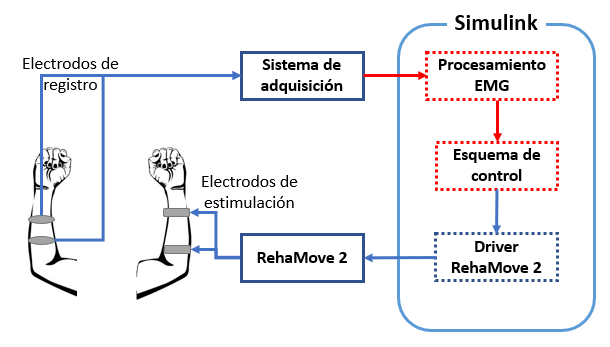
\includegraphics[scale=0.5]{SistemaPropuesto.png}
	\caption{Sistema propuesto para el proyecto. Líneas continuas representan entes de hardwares y líneas discontinuas representan entes de software.}
	\label{Figura: SistProp}
\end{figure}

Con la conclusión de este trabajo se espera que a futuro este sistema sea implementado para realizar un entrenamiento en espejo en sujetos que presenten hemiparesia. En este trabajo nos enfocaremos al desarrollo y evaluación del prototipo cuyo funcionamiento esperado es el siguiente: a través de los electrodos de registro se obtendrán dos canales de sEMG del miembro sano del sujeto, cada canal representará un movimiento (abrir mano y cerrar mano), dichos canales de EMG serán procesados para obtener dos parámetros, uno será el responsable de modular la intensidad de la corriente eléctrica que se aplicará al miembro con parálisis, y otro será un selector del canal de estimulación que estará activo (un canal para apertura de mano y otro canal para cierre). Acoplado a un objeto cilíndrico, que se le pedirá al sujeto intente alzar, estará un sensor de fuerza (presión), dicho sensor se encargará de mandar una señal de retroalimentación al esquema de control que servirá como indicador de si ya se ha logrado sujetar el objeto, una vez logrado esto la estimulación se quedará fija por 5 segundos para permitirle al sujeto levantar y manipular el objeto, y pasado dicho tiempo se continuará con la modulación de la intensidad de la corriente eléctrica utilizando un enfoque proporcional.

Para lograr la implementación del sistema se plantean las siguientes tareas a realizar:

\section{Decodificación de stream de datos en Simulink}
El prototipo de adquisición utiliza un ADS1299 de Texas Instruments para realizar la conversión analógica-digital, y un microcontrolador MSP432P401R es el responsable de configurar y transmitir a la computadora la información del ADS. Dicha información está organizada en un bus de datos de 27 bytes (los cuales están en complemento a dos) como se muestra en la Figura \ref{Figura: BusOut}. Con cada muestra recibida en la computadora se recibe un bus de 27 bytes, por lo cuál, para poder obtener la información leída por el ADS se tiene que decodificar el stream de datos recibido.

\begin{figure}[htbp]
\centering
	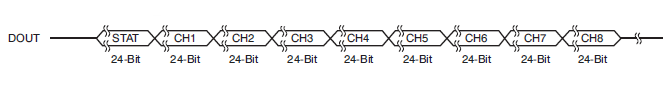
\includegraphics[scale=0.8]{Bus_Dat_Out_ADS.png}
	\caption{Estructura del bus de datos de salida del ADS1299}
	\label{Figura: BusOut}
\end{figure}

Para realizar la decodificación del stream de datos en Simulink, se utilizó el bloque \emph{Query Instrument} del \emph{Instrument Control Toolbox} para realizar la solicitud de datos al prototipo y se diseñó un subsistema utilizando bloques de la librería estándar de Simulink encargado de realizar la decodificación. Dicho subsitema sigue el funcionamiento mostrado en la Figura \ref{Figura: DecoStream}.\vfill

\begin{figure}[htbp]
\centering
	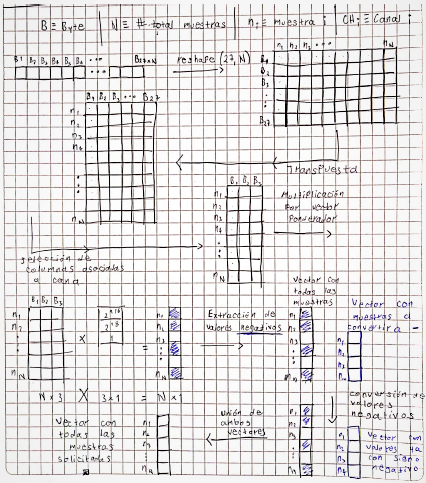
\includegraphics[scale=1.5]{Deco_Stream.png}
	\caption{Funcionamiento del subsistema decodificador del stream de datos}
	\label{Figura: DecoStream}
\end{figure}

\newpage
El funcionamiento del subsistema decodificador mostrado en la Figura~\ref{Figura: DecoStream} consiste en:
\begin{enumerate}
	\item Realizar la adquisición de N muestras, lo cual generará un vector columna con dimensión (27*N,1).
	\item Aplicar un reshape a dicho vector para obtener una matriz con dimensión (27,N).
	\item Obtener la transpuesta de dicha matriz para obtener una matriz con dimension (N,27).
	\item Para cada canal, extraer de la matriz anterior las columnas asociadas a dicho canal de tal forma que se obtenga una submatriz con dimensión (N,3).
	\item Realizar una multiplicación matricial de dicha submatriz con un vector ponderador de tal forma que al final se obtenga un vector con dimensión (N,1) donde cada muestra n se encuentra en complemento a 2.
	\item Extraer del vector anterior las muestras en las que se encuentra codificado un número negativo (si el bit 23 de la muestra es 1 entonces se trata de un número negativo).
	\item Obtener el complemento a 1 de cada muestra del subvector obtenido, sumar 1 a cada muestra y por último multiplicar cada muestra por -1.
	\item Regresar los elementos del subvector al vector original.
\end{enumerate}

En la Figura~\ref{Figura: DecoSimuT} se muestra el sistema implementado en Simulink que realiza los pasos anteriormente descritos para realizar la decodificación.

\begin{figure}[htbp]
	\centering
	\begin{subfigure}[htbp]{0.6\textwidth}
		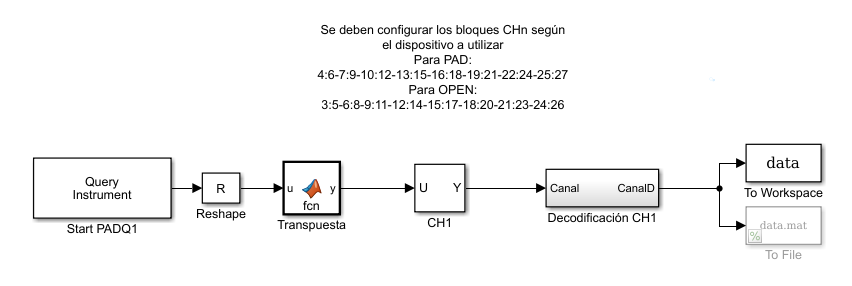
\includegraphics[width=\textwidth]{Read_Simu.png}
		\caption{Vista general del sistema diseñado para realizar la decodificación del stream de datos}
		\label{Figura: readSimu}
	\end{subfigure}
	\begin{subfigure}[htbp]{0.6\textwidth}
		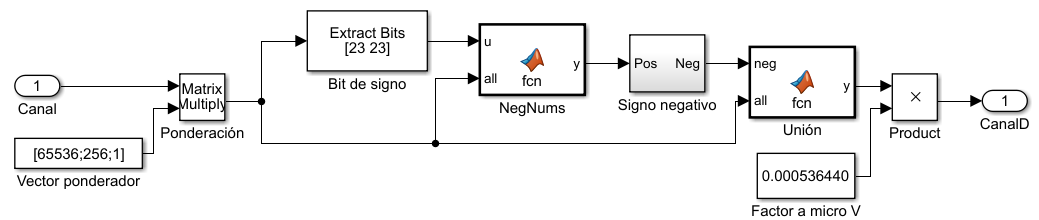
\includegraphics[width=\textwidth]{Deco_Simu.png}
		\caption{Vista interna del subsistema encargado de la decodificación de número negativos y positivos}
		\label{Figura: decoSimu}
	\end{subfigure}
	\caption{Sistema decodificador de stream de datos implementado en Simulink}
	\label{Figura: DecoSimuT}
\end{figure}

\newpage
\section{Evaluación de transferencia de datos entre prototipo de adquisición y computadora}
Debido a que el sistema de adquisición de bipotenciales se encuentra aún en una etapa de prototipo, se necesita saber si existe alguna perdida o alteración en las muestras adquiridas. Para esto, se propuso generar señales sintéticas en MATLAB que sirvieran como patrón para esta evaluación. Dichas señales consistieron en 5 senoidales con frecuencias de 1 Hz, 5 Hz, 10 Hz, 20 Hz y 50 Hz (Figura \ref{Figura: SenPur}), además de dos senoidales de 50 Hz moduladas en amplitud con una exponencial decreciente (Figura \ref{Figura: ExpAte}) y una recta con pendiente negativa (Figura \ref{Figura: LinAte}), por útlimo, una senoidal de 50 Hz modulada de tal forma que simule un contracción muscular que sube, se mantiene por un tiempo y baja (Figura \ref{Figura: Contra}). La duración de estas señales es de 5 segundos cada una, exeptuando la última que tiene una duración de 15 segundos, y todas se diseñaron con una frecuencia de muestreo de 1 kHz.

%Figura de senoidales MATLAB
\begin{figure}[htbp]
	\centering
	\begin{subfigure}[htbp]{0.4\textwidth}
		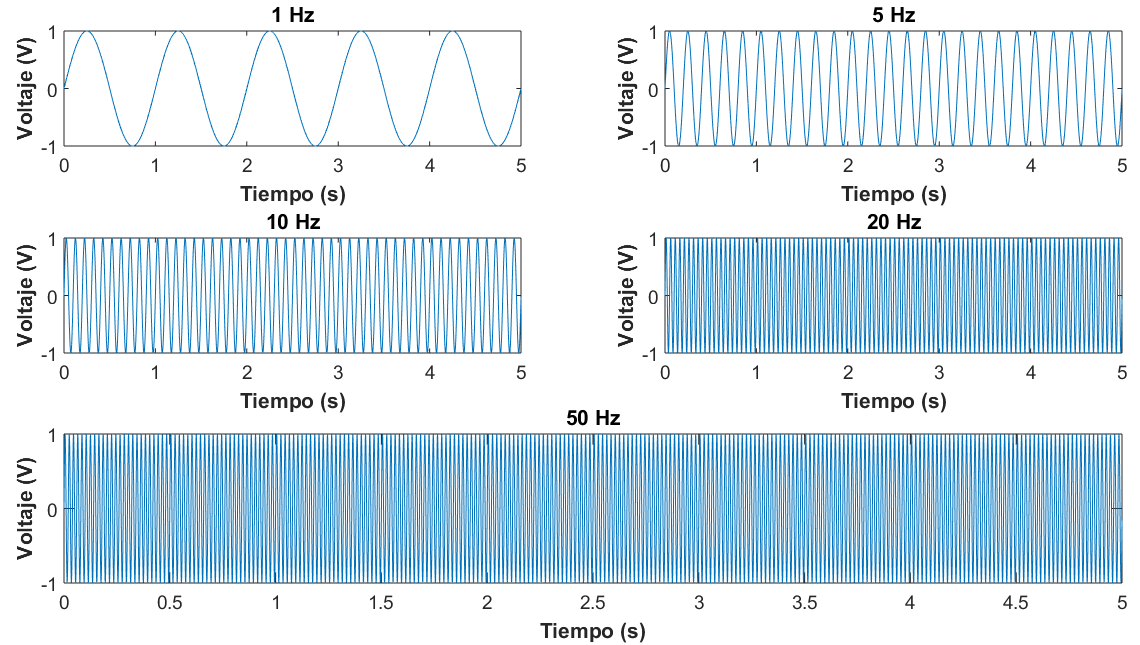
\includegraphics[width=\textwidth]{Sen_Pur.png}
		\caption{Senoidales puras a diferentes frecuencias}
		\label{Figura: SenPur}
	\end{subfigure}
	\hfill
	\begin{subfigure}[htbp]{0.4\textwidth}
		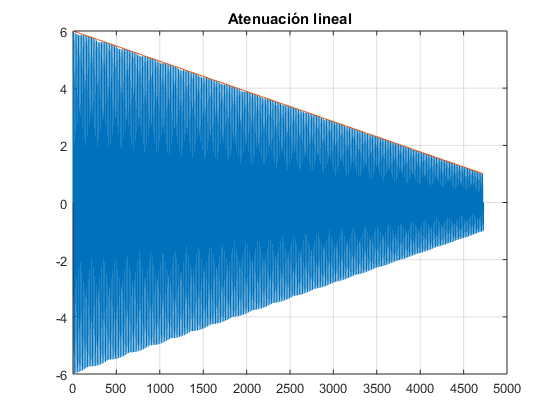
\includegraphics[width=\textwidth]{Lin_Ate.png}
		\caption{Senoidal de 50 Hz con atenuación lineal}
		\label{Figura: LinAte}
	\end{subfigure}
	\hfill
	\begin{subfigure}[htbp]{0.4\textwidth}
		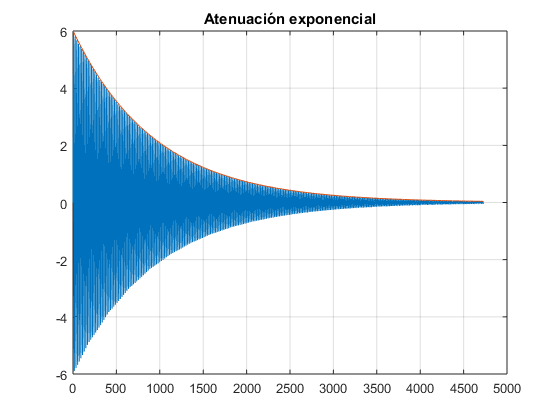
\includegraphics[width=\textwidth]{Exp_Ate.png}
		\caption{Senoidal de 50 Hz con atenuación exponencial}
		\label{Figura: ExpAte}
	\end{subfigure}
	\hfill
	\begin{subfigure}[htbp]{0.4\textwidth}
		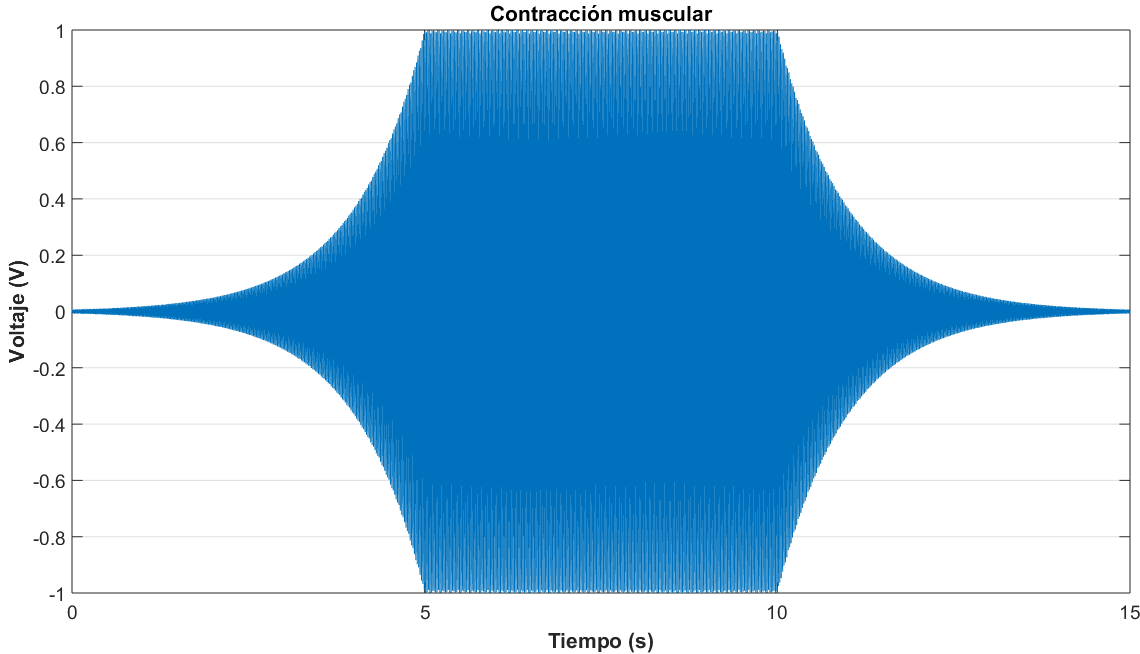
\includegraphics[width=\textwidth]{Contra.png}
		\caption{Senoidal de 50 Hz simulando una contracción muscular}
		\label{Figura: Contra}
	\end{subfigure}	
	\caption{Señales creadas para la evaluación del protocolo de comunicación}
	\label{Figura: SenalesEva}
\end{figure}

El proceso de evaluación se realizó de la siguiente manera:
\begin{itemize}
	\item Utilizando un jack de audio de 3.5 mm, se conectó una punta a la salida de audio de la computadora, mientras que la otra punta se conectó al canal 1 del prototipo de adquisición.
	\item El canal 1 del prototipo de adquisición se configuró con una ganancia de 1 y se hablilitó el BIAS para dicho canal. La frecuencia de muestreo del prototipo se configuró a 1 kHz.
	\item Se inició la solicitud de datos utilizando el subsistema decodificador implementado en Simulink y se inició el contento de un cronómetro.
	\item Tras haber transcurridos 2 segundo en el cronómetro, se procedió a la reproducción de la señal tratándola como una señal de audio.
	\item Al marcar el cronómetro 10 segundos (20 segundos para se señal de larga duración), se detuvo la adquisición en el sistema de Simulink.
	\item Se calculó la metrica de correlación entre ambas señales como indicador de la calidad de la transferencia de datos.
\end{itemize}

Estos pasos se repitieron tres veces para cada señal, esto para tener una mayor cantidad de datos con los cuales obtener una métrica de correlación promedio.

\section{Procesamiento de sEMG}
Se diseñarán filtros pasa banda que nos permitan tener información útil del sEMG como señal de control, la banda a utilizar aún está por definirse pero ya se cuentan con algunas opciones, las cuales son bandas que se han utilizado en otros trabajo que utilizan sEMG como señal de control \cite{Lenzi2012}\cite{Lenzi2011}\cite{Raafat}. Adicional a esto se diseñará un filtro rechaza banda para retirar el ruido de línea.

Para poder utilizar el sEMG como señal de control se tiene que utilizar algún descriptor de amplitud, siendo los más comúnes el valor rectificado promedio (ARV por sus siglas en Inglés) y el valor cuadrático medio (RMS por sus siglas en Inglés) \cite{Cavalcanti-Garcia2009}. Estos descriptores de amplitud se implementarán utilizando bloques estándar de Simulink y se valorará cuál puede proporcionar una señal de control más estable.

\section{Mapeo sEMG-FES}
Para poder convertir el descriptor de amplitud de sEMG se planea realizar un mapeo que convierta los valores del descriptor a valores de amplitud de la corriente eléctrica que proporcionará el dispositivo de estimulación eléctrica. Para esto, se planea utilizar un mapeo lineal utilizando una ecuación de una recta cuyos parámetros se definirán tras una etapa de calibración del sistema.

\section{Implementación de sensor de fuerza}
Se acoplará un sensor de fuerza a un objeto cilíndrico, como una botella o un vaso, el cual nos servirá como indicador de la fuerza que se le está aplicando al objeto. Dicho sensor estará acompañado de una etapa de procesamiento, la cual consistirá en una función que, tras pasar un umbral de fuerza predefinido en la calibración, enviará una señal de retroalimentación que le indicará al esquema de control en lazo cerrado, que se ha logrado sujetar el objeto; midiendo continuamente la presión y utilizando esta información para indicar al sistema de control si se mantiene la estimulación o tiene que ser modulada.

\section{Desarrollo de esquema de control}
El esquema de control consistirá en la modulación de la estimulación eléctrica a partir del descriptor de amplitu de sEMG que se decida usar, esta intensidad tendrá un valor mínimo y máximo que serán definidos por nosotros previos a iniciar las pruebas del sistema terminado. Inicialmente se propuso utilizar un sensor de fuerza como señal de retroalimentación que indique el momento en el que se ha logrado la fuerza suficiente para levantar el objeto, pero se está considerando otra alternativa en la cual ya no se utilizaría el sensor de fuerza y quién serviría como retroalimentación sería el mismo sujeto de prueba.